\documentclass[12pt]{article}
\usepackage{geometry}                % See geometry.pdf to learn the layout options. There are lots.
\geometry{a4paper}                   % ... or a4paper or a5paper or ... 
\usepackage{graphicx}
\usepackage{amssymb}
\usepackage{amsthm}
\usepackage{epstopdf}
\usepackage[utf8]{inputenc}
\usepackage[gen]{eurosym}
\usepackage[usenames,dvipsnames]{color}
\usepackage[table]{xcolor}
\usepackage{hyperref}
\DeclareGraphicsRule{.tif}{png}{.png}{`convert #1 `dirname #1`/`basename #1 .tif`.png}

\theoremstyle{definition}
\newtheorem{example}{Example}

\newenvironment{explanation}{%
   \setlength{\parindent}{0pt}
   \itshape
   \color{blue}
}{}

\newcommand{\projectname}{Nao Soccer}
\newcommand{\productname}{Nao States}
\newcommand{\projectleader}{Viktoria Streibl, Melanie Mühleder, Sabina Brantner}
\newcommand{\documentstatus}{In progress}
%\newcommand{\documentstatus}{Submitted}
%\newcommand{\documentstatus}{Released}
\newcommand{\version}{V. 1.0}
\newcommand{\unclear}[1]{\vspace{.5em}\parbox{.9\linewidth}{\color{red}{\bf Remark: #1}}\vspace{.5em}}

\begin{document}
\begin{titlepage}
\begin{flushright}

\includegraphics[scale=.5]{htlleondinglogo.png}\\
\end{flushright}

\vspace{10em}

\begin{center}
{\Huge Design Document} \\[3em]
{\LARGE \productname} \\[3em]
\end{center}

\begin{flushleft}
\begin{tabular}{|l|l|}
\hline
Project Name & \projectname \\ \hline
Project Leader & \projectleader \\ \hline
Document state & \documentstatus \\ \hline
Version & \version \\ \hline
\end{tabular}
\end{flushleft}

\end{titlepage}
\section*{Revisions}
\begin{tabular}{|p{.25\linewidth}|p{.3\linewidth}|p{.37\linewidth}|}
\hline
\cellcolor[gray]{0.5}\textcolor{white}{Date} & \cellcolor[gray]{0.45}\textcolor{white}{Author} & \cellcolor[gray]{0.5}\textcolor{white}{Change} \\ \hline
August 17, 2016&V. Streibl, M. Mühleder, S. Brantner&First version \\ \hline
\end{tabular}
\pagebreak

\setcounter{tocdepth}{2}
\tableofcontents
\pagebreak

\section{Introduction}\label{sec:managementsummary}

\section{Show Robot Status}
To quickly monitor the status of the Naos, we plan to implement some status indicators via coloring its eyes. The following table represents some first ideas which status could be interesting to facilitate our development and how we want to indicate with two eyes colors.
\\[1em]
\unclear{In the next table: What is if the Nao sees the goal? What means the red/red status? What do you mean by ``the x/y state is necessary?}
\\
\unclear{Please check if the state diagram is okay, and the table beneath}\\
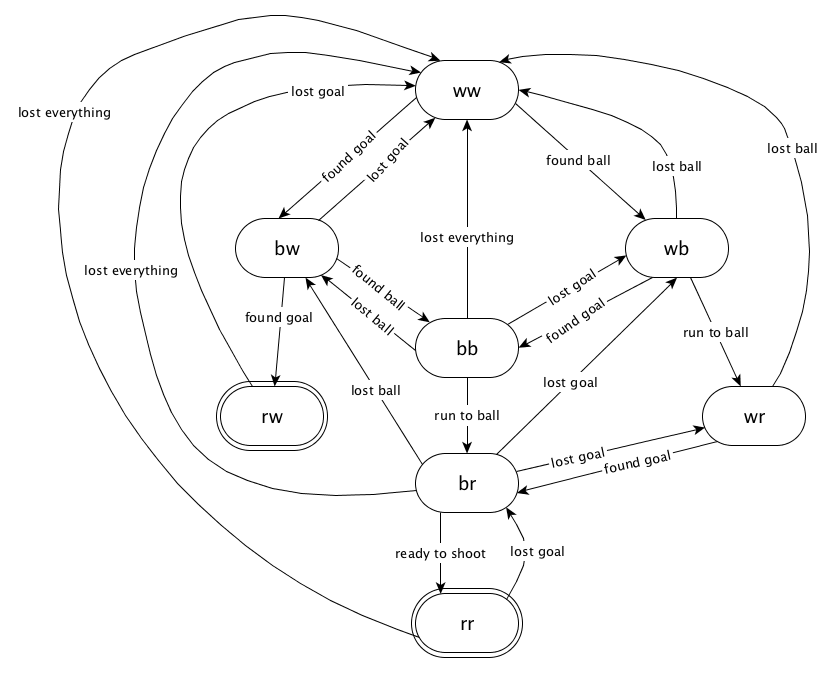
\includegraphics[scale=.5]{stateDiagram.png} 

\begin{tabular}{|p{.21\linewidth}|p{.3\linewidth}|p{.38\linewidth}|}
\hline
\cellcolor[gray]{0.5}\textcolor{white}{Shortcut} & \cellcolor[gray]{0.45}\textcolor{white}{Meaning} & \cellcolor[gray]{0.5}\textcolor{white}{Status}\\ \hline
ww&Left and right eye are white&The Nao can't see the ball or the goal\\ \hline
bw&Left eye blue, right eye white&The Nao has found the goal but no ball \\ \hline
bb&Left and right eye are blue&Has found goal and ball, but to far away for kick \\ \hline
wb&Left eye white, right eye blue&The Nao has found the ball but not the goal\\ \hline 
rw&Left eye red, right eye white&Nao tells other teammates where the goal is \\ \hline
br&Left eye blue, right eye red&The Nao has the ball and found the goal and it is on the way to the ball\\ \hline
wr&Left eye white, right eye red&The Nao plans to access the ball, this is only possible if the left eye was blue before\\ \hline
rr&Left and right eye are red&The Nao kick the ball to the goal, only after the blue-red status\\ \hline
\end{tabular}

\bibliography{my_bibliography}{}
\bibliographystyle{plainurl} % save alternatives are abbrvurl	alphaurl	plainurl	unsrturl
\end{document}  